\documentclass{beamer}
\usepackage{amsfonts}
\usepackage{amsmath}
\usepackage{amssymb}
\usepackage{graphicx}
\usepackage{subfigure}
\usepackage{mathrsfs}
\usepackage{algorithm,algorithmic}

\usetheme{default}
\begin{document}

\title{Extracting User's Hidden Profile on Twitter}
\author{Dong Wang, Mohan Yang, Yuchen Liu}
\institute{Department of Computer Science\\University of California, Los Angeles}
\date{Nov 21, 2011}

\newcommand{\following}{\ensuremath{following}}
\newcommand{\follower}{\ensuremath{follower}}
\newcommand{\at}{\emph{@}}


\begin{frame}
  \titlepage
\end{frame}

\AtBeginSection[] % Do nothing for \section*
{
\begin{frame}<beamer> \frametitle{Extracting User's Hidden Profile on Twitter}
\tableofcontents[currentsection]
\end{frame}
}

\section{Introduction}
\begin{frame}{Introduction}
123
\end{frame}

\section{Problem Formulation}
\begin{frame}{Problem Formulation}
\begin{itemize}
\item A directed graph $G = (V,E)$
\item A node $u \in V = \{1, 2, \cdots, n\}$ represents a user in twitter
\item A directed edge $(u,v) \in E$ indicates user $u$ is following user $v$
\item Sets $\follower(u)$ and $\following(u)$
\item Size of set is $|\follower(u)|$, and $|\following(u)|$
\end{itemize}
\pause

\begin{itemize}
\item A category $\mathcal{C}$, we want to identify all users that belong to $\mathcal{C}$
\item Prior knowledge, $V = \mathcal{A} + \mathcal{B}$
\begin{itemize}
\item Users in $\mathcal{A}$ belong to $\mathcal{C}$
\item The results for users in $\mathcal{B}$ are unknown
\end{itemize}
\item A relevance score $s_u$ for $u \in \mathcal{B}$, rank users in $\mathcal{B}$ based on $s_u$
\end{itemize}
\end{frame}

\section{Our Approach}
\begin{frame}{Snowball Algorithm}
\begin{itemize}
\item The probability of a user $u$ belonging to $\mathcal{C}$ is determined by the relevance score $s_u$
\item Assume the probability of $u$ publishing a tweet belonging to $\mathcal{C}$ is also $s_u$, and each user publishes the same number ($k$) of tweets
\item The probability of receiving a tweet in $\mathcal{C}$ by $u$ is
$${\sum_{v \in \following(u)} s_v k \over |\following(u)|k} = \sum_{v \in following(u)}{s_v \over |\following(u)|}$$
\item Further assume that a user publishes exactly what he receives, then the probability of publishing a tweet in $\mathcal{C}$ by $u$ is
$$s_u = \sum_{v \in \following(u)} \frac{s_v}{|\following(u)|}$$
\end{itemize}
\end{frame}

\begin{frame}{Bidirectional Snowball Algorithm}
\begin{itemize}
\item Snowball - tweets propagation from user to his \alert{followers}
\item Inverse direction - tweets propagation from user to his \alert{followings}
\item A user in $\mathcal{C}$ tends to follow many users in $\mathcal{C}$, while a user followed by many users in $\mathcal{C}$ tends to belong to $\mathcal{C}$
\begin{eqnarray}\label{eq:bidsnowball}
p_u & = & \sum_{v \in \following(u)} \frac{p_v}{|\following(u)|} \nonumber \\
q_u & = & \sum_{v \in \follower(u)} \frac{q_v}{|\follower(u)|} \nonumber
\end{eqnarray}
\item Users are ranked according to the relevance score $s_u = p_u q_u$, which is a combination of relevance to category $\mathcal{C}$ from both following and follower directions
\end{itemize}
\end{frame}

\begin{frame}{Naive Bayes Algorithm}
\begin{itemize}
\item Users in $\mathcal{A}$ ($\mathcal{B}$) are positive (negative) training examples
\item $T_u$ is the collection of $u$'s tweets, location and biography
\item $W = \{w_1, \cdots, w_m\}$ is the word set for corpus $\bigcup_{u = 1}^n T_u$
\item $\mathbf{1}_{T_u}(w_i)$ is the indicator function of $T_u$
\pause
\item The naive Bayes classifier finds $i \in \{0, 1\}$ which maximizes
$$p(c = i | w_1 = \mathbf{1}_{T_u}(w_1), \cdots, w_m = \mathbf{1}_{T_u}(w_m)),$$
\item or equivalently maximizes
$$p(c = i) \prod_{j=1}^m p(w_j = \mathbf{1}_{T_u}(w_j) | c = i).$$
\item It is equivalent to determining the sign for $s_u$
\begin{eqnarray}
s_u & = & \log(p(c = 1)) - \log(p(c = 0)) \nonumber \\
    & + & \sum_{j=1}^m (p(w_j = \mathbf{1}_{T_u}(w_j)|c = 1) - p(w_j = \mathbf{1}_{T_u}(w_j)|c = 0)). \nonumber
\end{eqnarray}
\end{itemize}
\end{frame}

\begin{frame}{Co-training Algorithm}
\begin{block}{Perspective of previous algorithms}
\begin{itemize}
\item Bidirectional snowball algorithm - network structure level
\item Naive Bayes algorithm - tweets information level
\end{itemize}
\end{block}
\pause
Co-training algorithm combines the two algorithms together, iteratively reinforce the result of one algorithm by the result of the other algorithm.
\end{frame}

\begin{frame}{Co-training Algorithm}
\begin{algorithm}[H]
\caption{\textsc{Co-training}}
\textbf{Input: }{Category $\mathcal{C}$, two disjoint sets $\mathcal{A}$ and $\mathcal{B}$, parameter $k$ and $l$}\\
\textbf{Output: }{An array $rank$ containing users in $\mathcal{B}$ ranked on the probability of belonging to $\mathcal{C}$}
\begin{algorithmic}[1]
\REPEAT
\STATE $rank^{\prime}$ $\leftarrow$ bidirectional snowball algorithm($\mathcal{A}$, $\mathcal{B}$)
\STATE $rank$ $\leftarrow$ naive Bayes algorithm($\mathcal{A}$, $\mathcal{B}$)
\STATE $\mathcal{A} \leftarrow \mathcal{A} ~ + $ \{top $l$ users in $rank^{\prime}$\}
\STATE $\mathcal{A} \leftarrow \mathcal{A} ~ + $ \{top $l$ users in $rank$\}
\UNTIL{Top $k$ users in $rank^{\prime}$ and $rank$ are the same}
\RETURN $rank$
\end{algorithmic}
\label{alg:cotrain}
\end{algorithm}
\end{frame}

\section{Experiments}
\begin{frame}{Experiment Setup}
\begin{itemize}
\item Data collection
\begin{itemize}
\item Seed users from UCLA, USC, Stanford and MIT, two-level breadth first traversal starting from seed user
\item $540,000$ users, $15,321,508$ tweets, $3,143,115$ different words
\item Filter out less frequent words(occurrance $<$ 100) $=>$ about $20,000$ words
\end{itemize}
\item Category $\mathcal{C}$ and keyword $z_{\mathcal{C}}$ $=>$ $V = \mathcal{A} + \mathcal{B}$
\begin{itemize}
\item $\mathcal{C} = $ ``users in UCLA'', $z_{\mathcal{C}} = $ ``UCLA''
\end{itemize}
\item Randomly select $20\%$ from $\mathcal{A}$, remove the bigoraphy and move them to $\mathcal{B}$
\item Manually label top 100 results of different methods for UCLA category
\end{itemize}
\end{frame}

\begin{frame}{Precision\at$k$ for UCLA Category}
\begin{center}
  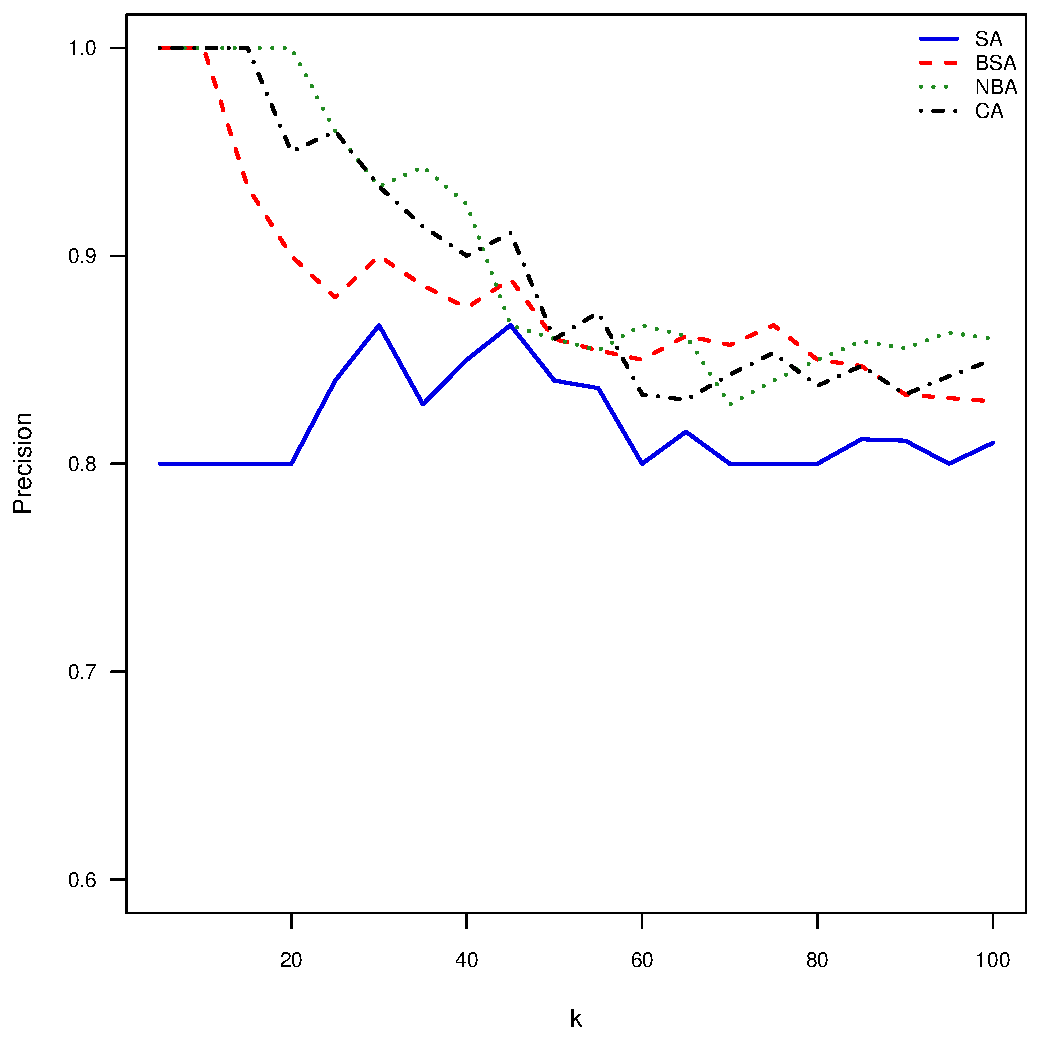
\includegraphics[width=200pt]{experiment/e1_ucla.pdf}  
\end{center}
\end{frame}

\begin{frame}{Precision\at$k$ for USC Category}
\begin{center}
  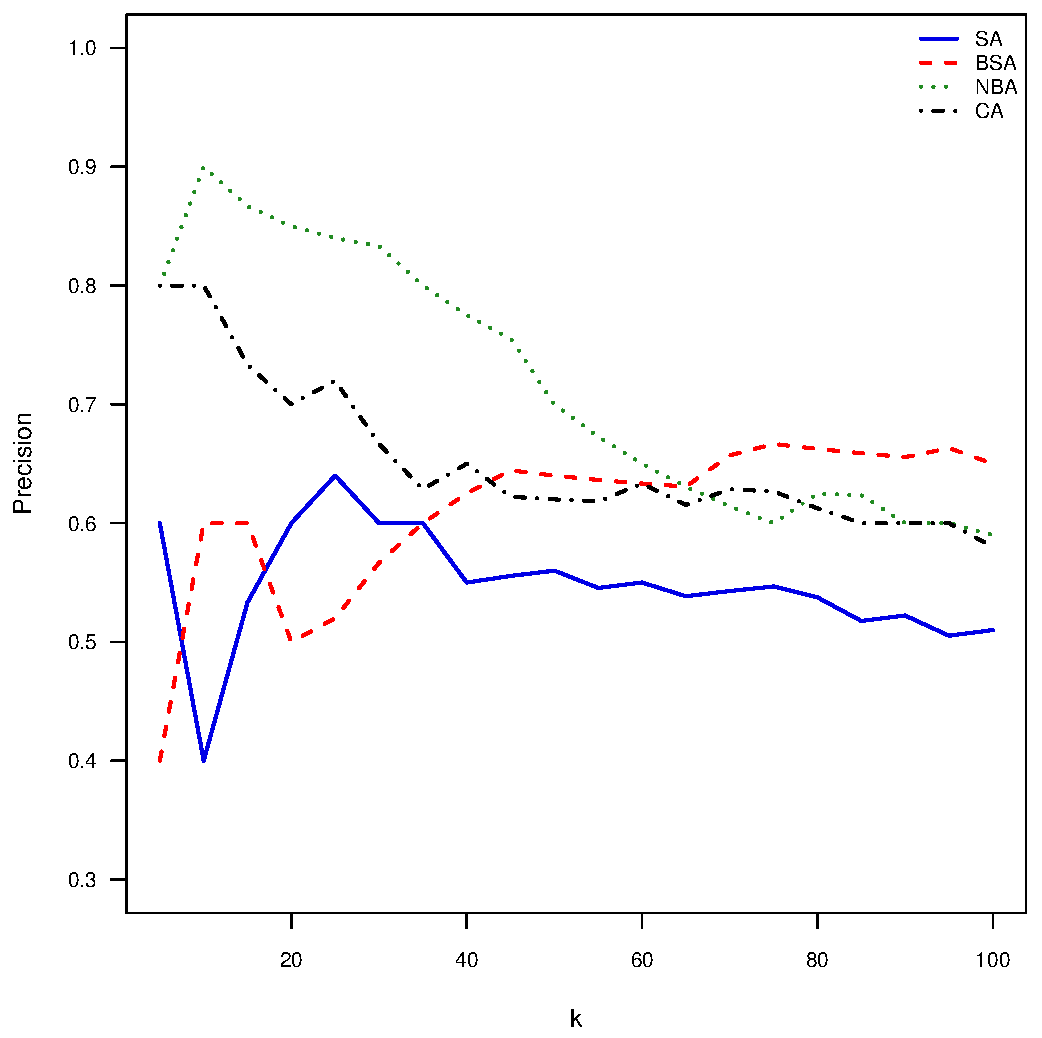
\includegraphics[width=200pt]{experiment/e1_usc.pdf}
\end{center}
\end{frame}

\begin{frame}{Precision\at$k$ for Stanford Category}
\begin{center}
  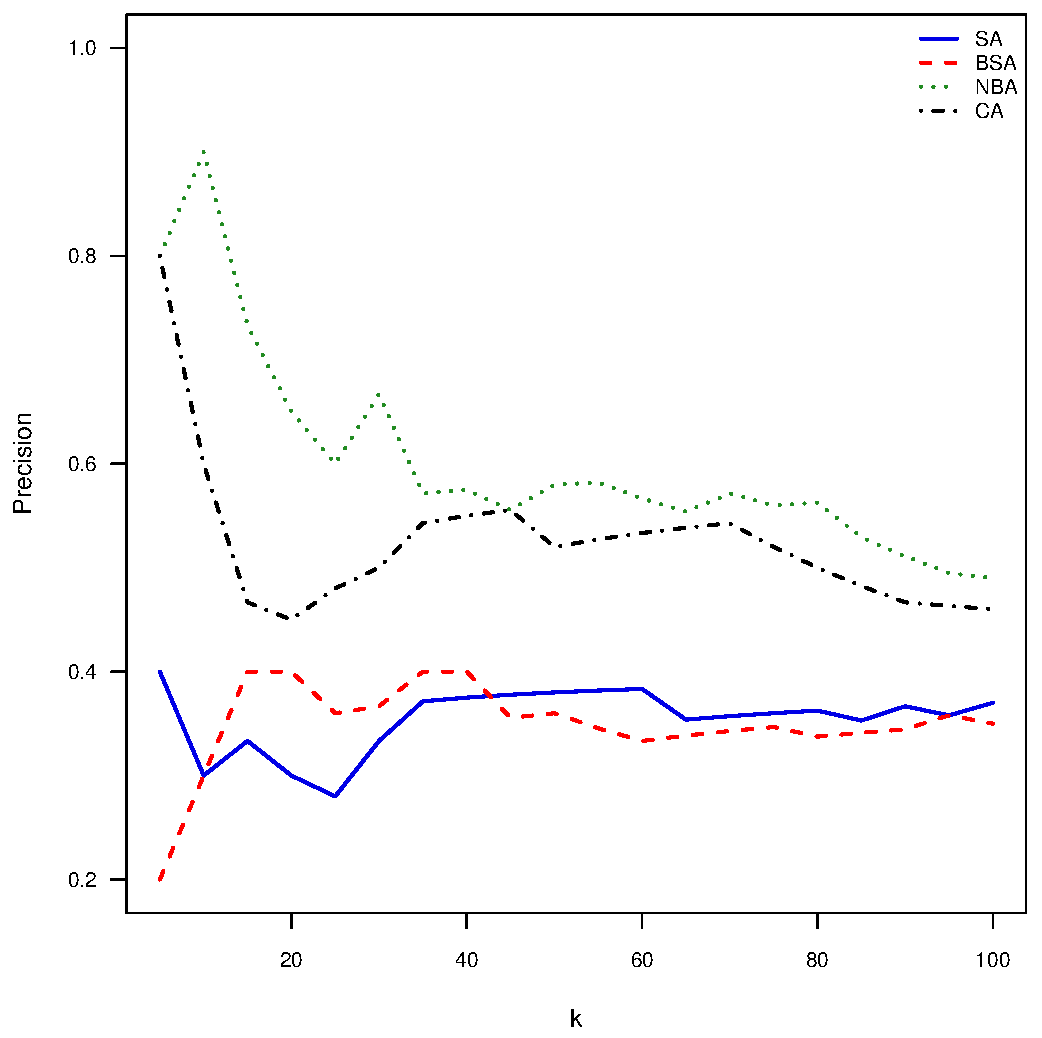
\includegraphics[width=200pt]{experiment/e1_stanford.pdf}
\end{center}
\end{frame}

\begin{frame}{Precision\at$k$ for MIT Category}
\begin{center}
  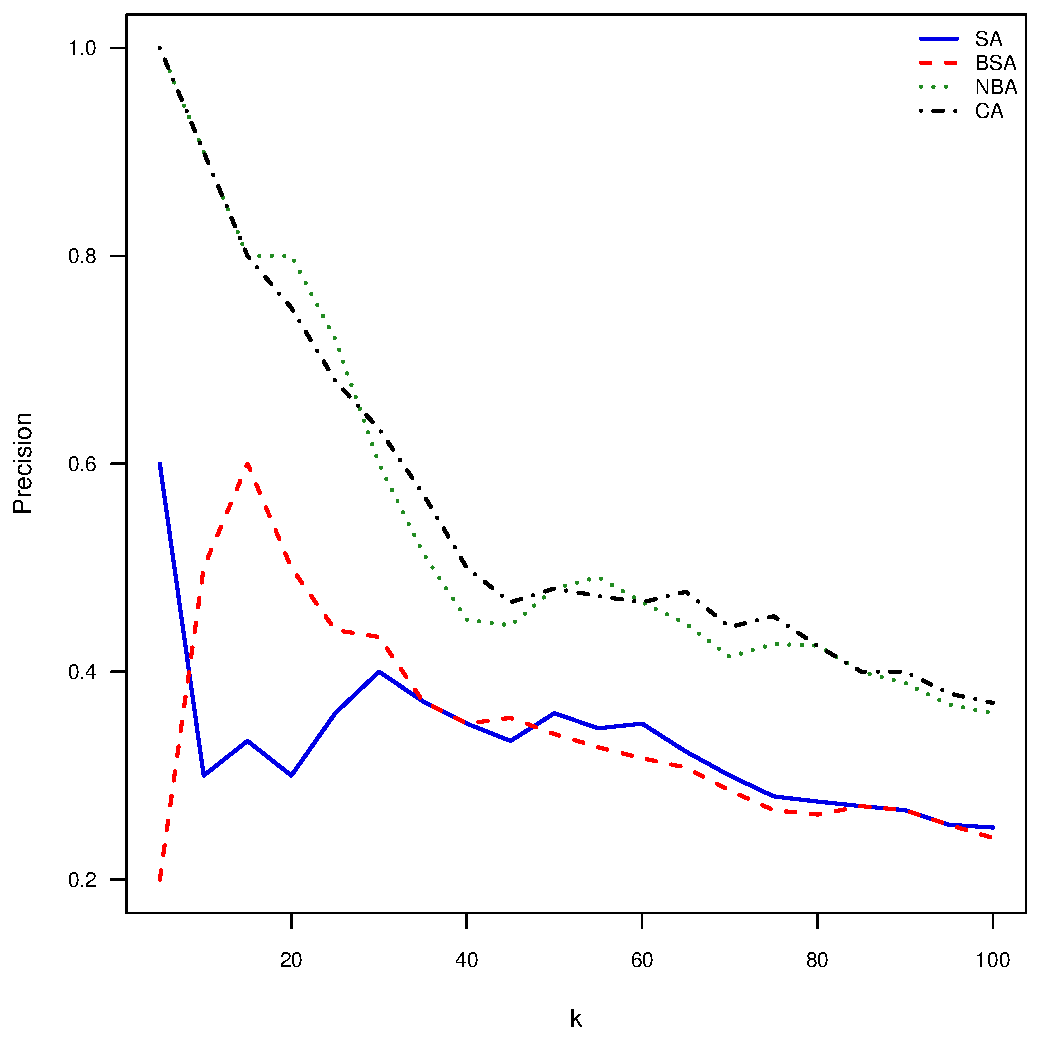
\includegraphics[width=200pt]{experiment/e1_mit.pdf}
\end{center}
\end{frame}

\begin{frame}{Human Labeled Data Vs. Automatic Evaluation}
\begin{columns}[c]
\column{2in}
  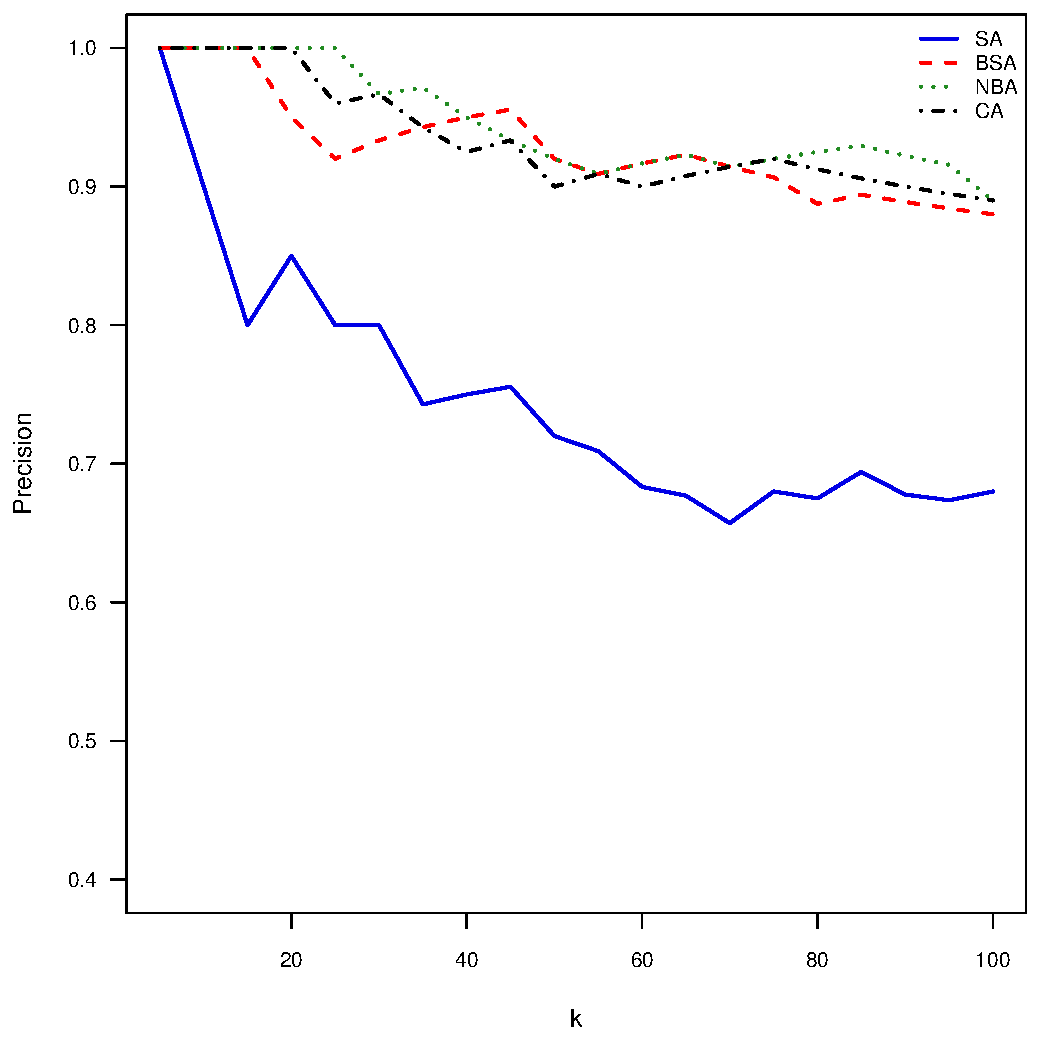
\includegraphics[width=2in]{experiment/e1_ucla_pool.pdf}
  \begin{center}Precision\at$k$ for UCLA category on human labeled data\end{center}
\column{2in}
  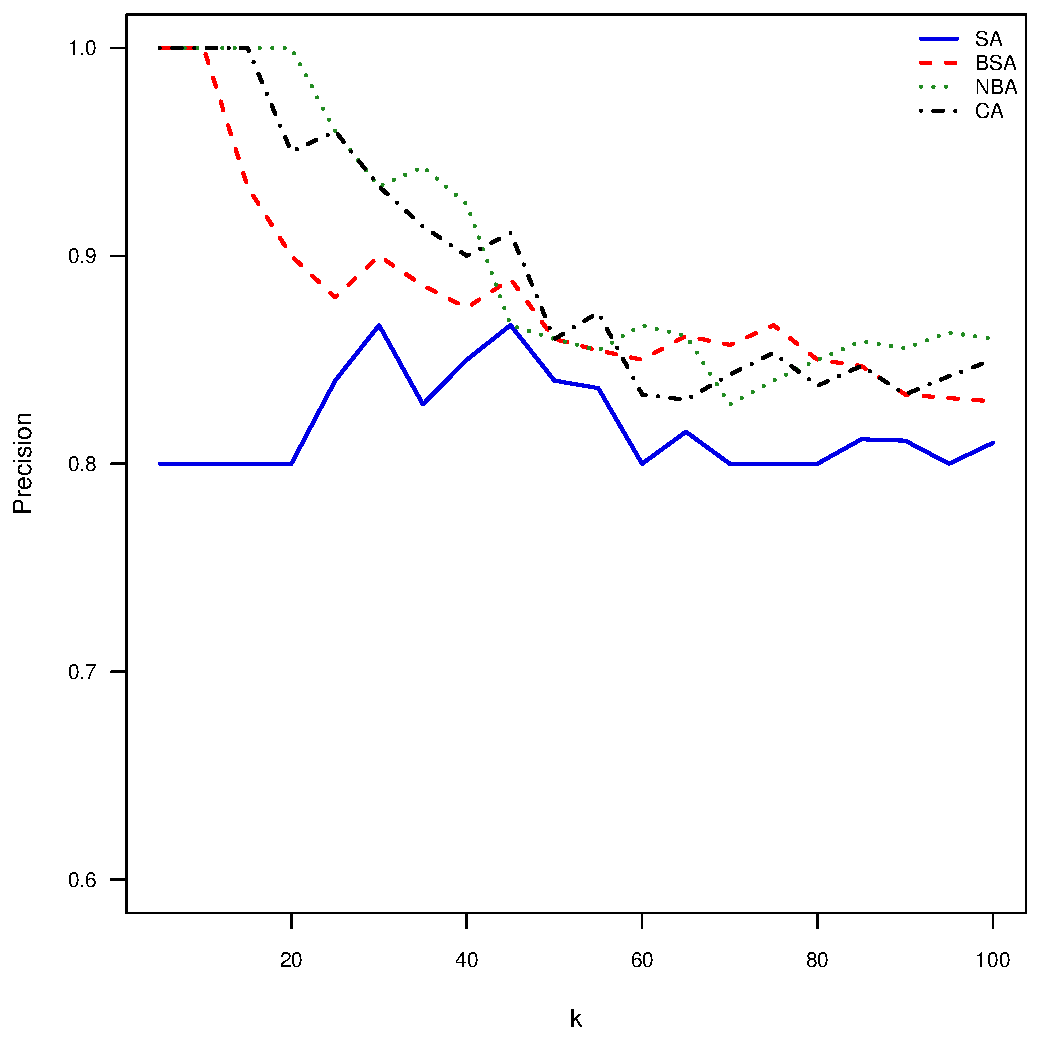
\includegraphics[width=2in]{experiment/e1_ucla.pdf}
  \begin{center}Precision\at$k$ for UCLA category with automatic evaluation\end{center}
\end{columns}
\end{frame}

\begin{frame}{Precision\at$k$ for UCLA Category With Loss of Information}
\begin{center}
  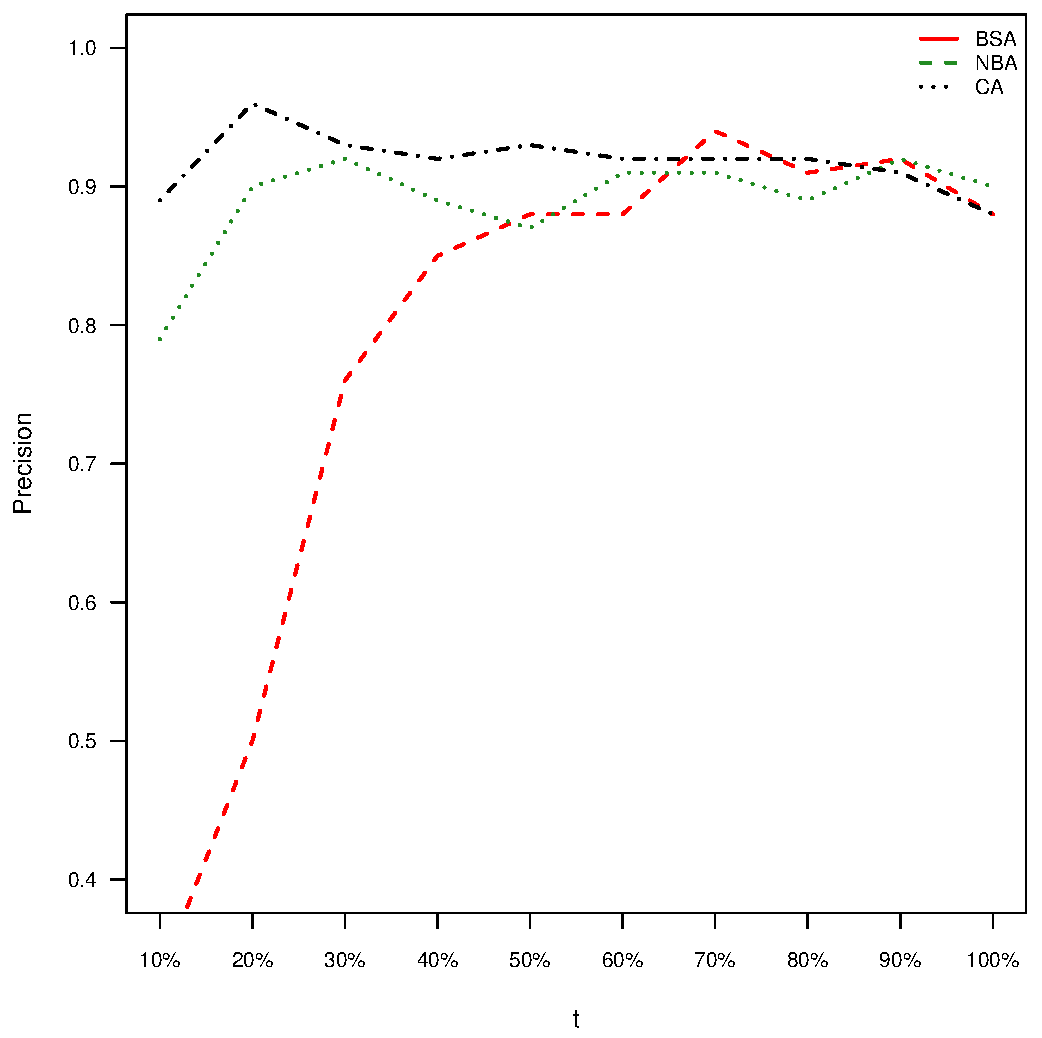
\includegraphics[width=200pt]{experiment/e2_ucla.pdf}
\end{center}
\end{frame}


\section{Dicsussion}
\begin{frame}{User Classification}
\begin{center}
  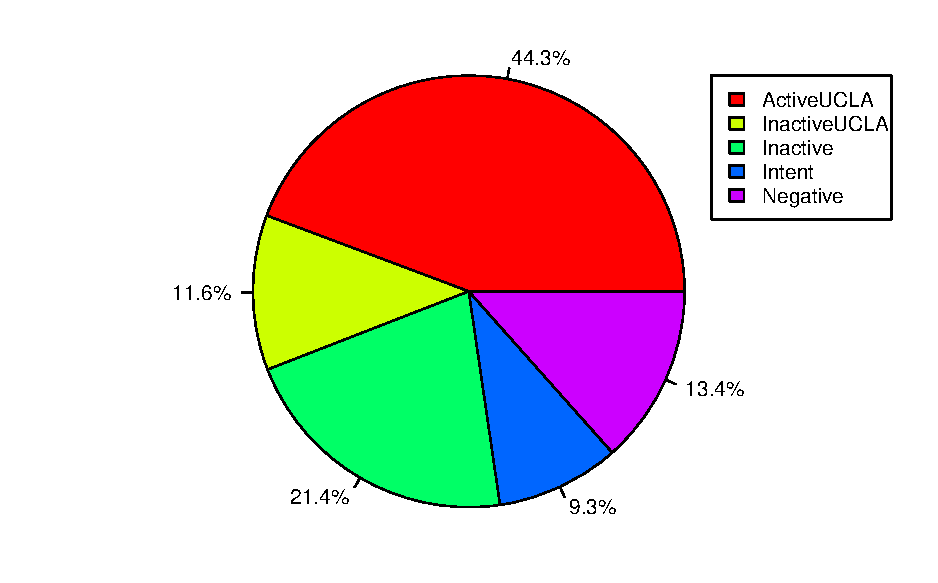
\includegraphics[width=300pt]{experiment/uc.pdf}
\end{center}
\end{frame}

\begin{frame}{Precision\at$k$ of Active Users in UCLA Category}
\begin{center}
  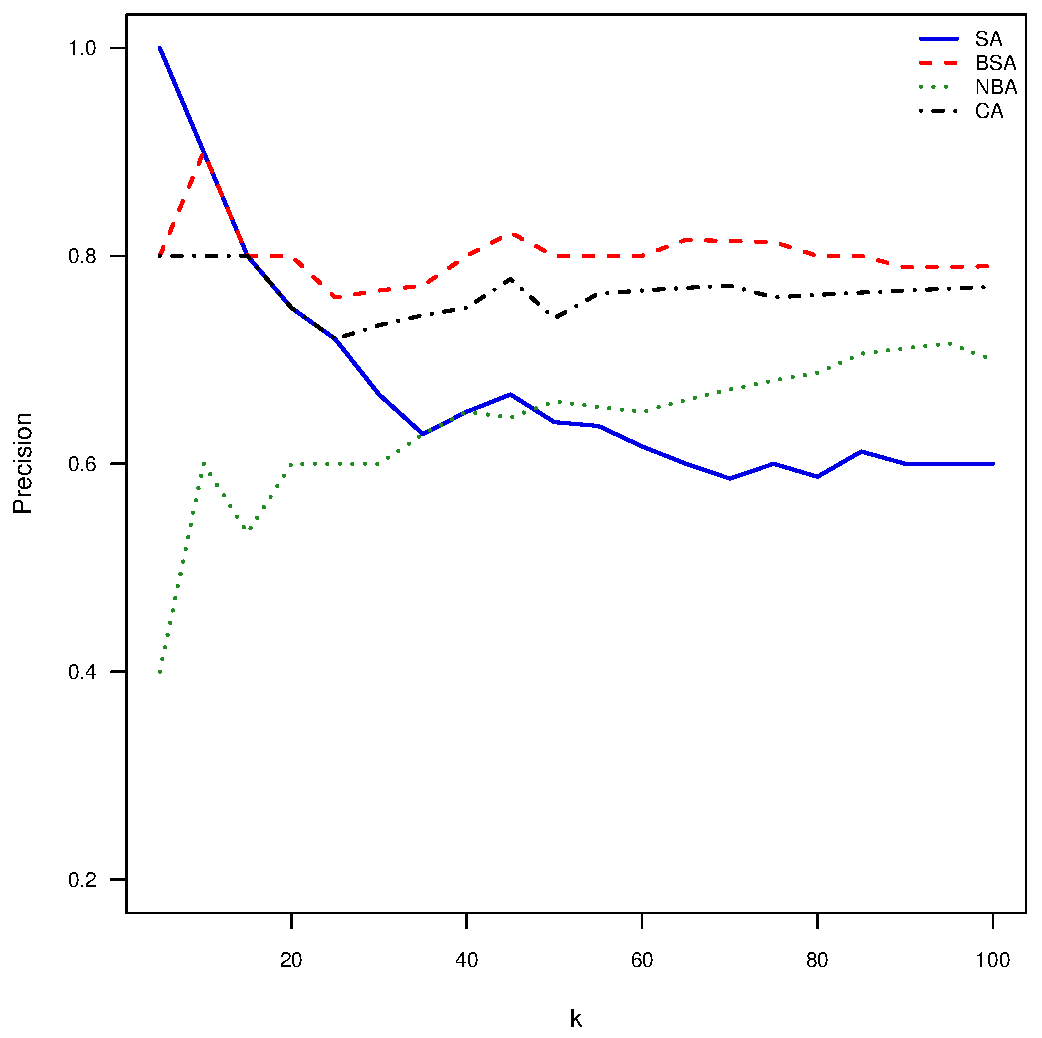
\includegraphics[width=200pt]{experiment/ap.pdf}
\end{center}
\end{frame}

\section{Conclusion}
\begin{frame}{Conclusion}
saasdas
\end{frame}

\begin{frame}{}
\begin{center}
{\Huge Thanks!}
\end{center}
\end{frame}

\end{document}
